\chapter{System Design}
\label{chap:3}

In this chapter, the overall system design is discussed. The chapter is divided up into 
six sections with each section focusing on a different aspect of the complete
system. These six sections are:

\begin{enumerate}
  \item The vending machine central controller.
  \item The Near Field Communication controller.
  \item The Quick Response Code camera.
  \item The product dispensing mechanism.
  \item The vending machine unit.
  \item The encryption scheme used.
\end{enumerate}

Each section explains which technology or service was used in the final
component design.

Where two or more available services or technologies were available,
a brief discussion and explanation is given as to why the particular technology or
service was used in the final design of the vending machine.

\section{System Overview}

Figure \ref{fig:system-overview-pi} gives a diagrammatical layout of the complete system.
It shows the interactions between the different sub-components of the complete system.

\begin{figure}
\centering
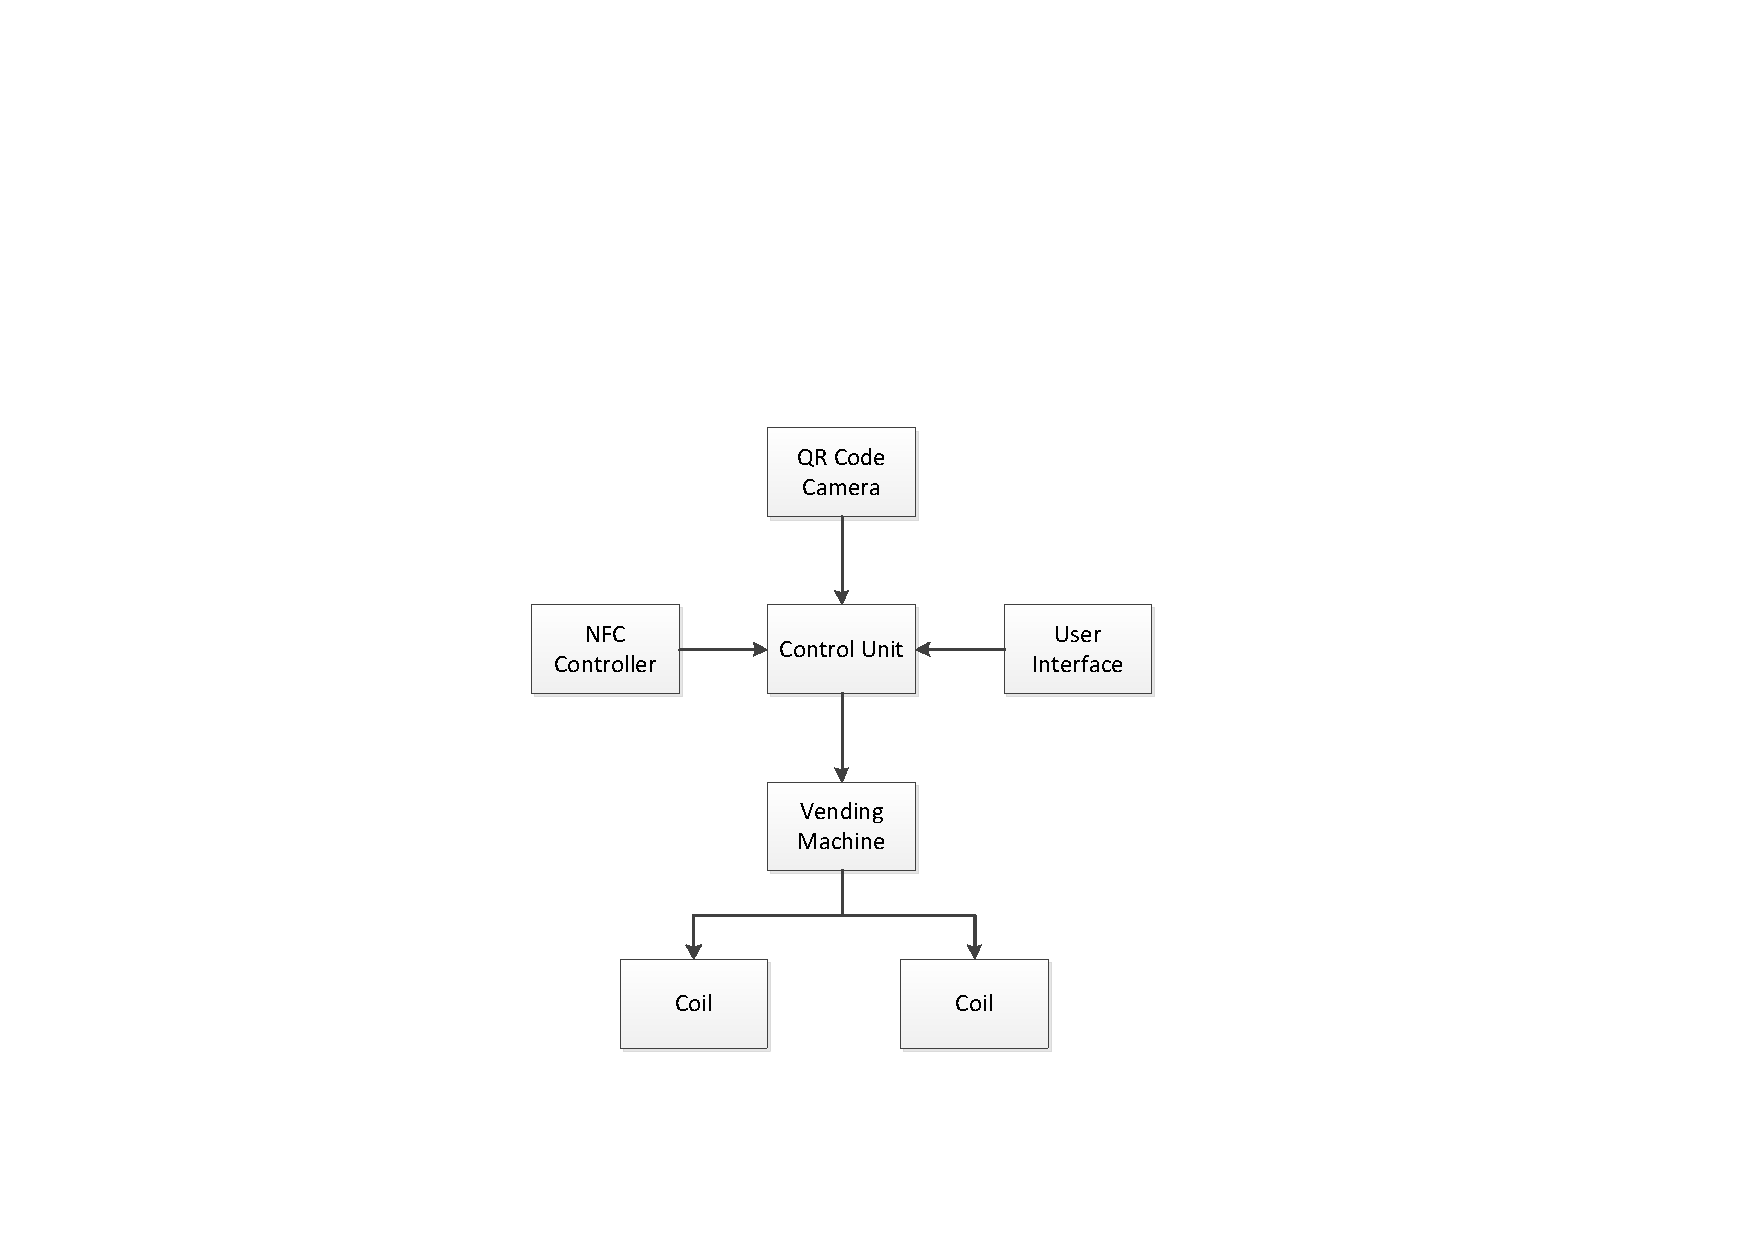
\includegraphics[clip=true, trim = 100 80 0 150, scale=0.7]{pi_system_overview}
\caption{System overview from the control unit's perspective.}
\label{fig:system-overview-pi}
\end{figure}

The components used in these subsystems are discussed in the subsequent sections of this
chapter.

\section{Central Control Unit}

To be able to handle the image processing that QR Code decoding and NFC handling requires, a
relatively powerful central controller is required. Although there are many controllers capable
of this, only two main alternatives were considered in this project. They are the
Raspberry Pi microcomputer and the Arduino Uno microcontroller.

These controllers are discussed in this section.

\subsection{Arduino Uno}

The Arduino Uno is popular open-source microcontroller (see Figure
\ref{fig:arduino}). It is based on an 8-bit Atmel ATmega328 ARM microprocessor.
Its official specifications are given in Table \ref{tab:arduino-specs}.

\begin{figure}
\centering
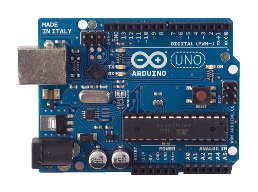
\includegraphics[scale=1.5]{arduino.eps}
\caption[Picture of an Arduino Uno microcontroller.]{Picture of an Arduino Uno
microcontroller [\cite{manual:arduino-specs}].}
\label{fig:arduino}
\end{figure}

\begin{table}
\centering
\caption{Arduino Uno Specs[\cite{manual:arduino-specs}].}
  \begin{tabular}{|l|l|}
  \hline
    Operating Voltage & 5 V \\\hline
    Processor & Atmel ATmega328 (clocked at 16 MHz) \\\hline
    GPIO Pins & 14 (6 of which are Pulse Width Modulator enabled) \\\hline
    Memory & 32 kB Flash, 2kB SRAM, 1kB EEPROM \\\hline
    Communication & i$^2$c, UART, SPI \\\hline
    Price & R310.00 \\\hline
  \end{tabular}
  \label{tab:arduino-specs}
\end{table}

Because of its open-source design, there are a multitude of peripheral devices and expansion
boards (known as `shields'), along with all their libraries and drivers,
available locally. The Arduino's programming language of choice is a modified version of
C and comes with its own Integrated Development Environment (IDE). This, along
with its relatively low cost and specifications, makes the Arduino Uno
an attractive option for this project.

\subsection{Raspberry Pi}
\label{sec:raspi}

The Raspberry Pi is a Debian Linux-based microcomputer
designed and manufactured by a UK-based charity called the Raspberry Pi Foundation, for the
purpose of educating and familiarising young children with programming. However, its low price
and respectable specifications makes it a strong choice as a control unit for the vending
machine.

The Pi was designed with the focus on Python as its main programming language, which makes
running scripts and controlling the board relatively simple. It also runs on a modified
version of Debian Linux called Raspbian.

Its main specifications are given in Table \ref{tab:rpi-specs}.

\begin{table}
\centering
\caption{Raspberry Pi Specifications [\cite{website:raspi-specs}].}
  \begin{tabular}{|l|l|}
  \hline
  Operating Voltage & 3.3 V \\\hline
  Processor & ARM 6 clocked at 700 MHz \\\hline
  GPIO Pins & 28 Pins \\\hline
  Memory & 512 MB RAM \\\hline
  Communication & SPI, UART, USB, i$^2$c, Ethernet \\\hline
  Price & R400.00 \\\hline
  Video & HDMI Output \\\hline
  \end{tabular}
  \label{tab:rpi-specs}
\end{table}

\subsection{Design Choice}

The Raspberry Pi was chosen to be used as the central controller of this project and
controls the hardware connected to it via a Universal Serial Bus (USB) connection, or one of
its General Purpose Input Output (GPIO) pins.

The Pi was chosen ahead of the Arduino, mainly because of its video stream processing capabilities 
and that libnfc can be installed on it. This allows the Pi to decode QR Codes and to communicate with 
an NFC-enable cellphone. Furthermore, the Pi can interface with desktop peripheral hardware, such as a mouse and
keyboard, which made development and prototyping much simpler.

After development and optimisation has been completed for this project, work can begin on porting it to 
a micro-controller, such as an Arduino. However, for the development phase of this project,
 the Pi is much better suited platform.

\section{NFC Controller}
\label{sec:nfc-controller}

The NFC controller that was selected is the PN532 NFC shield from Adafruit Industries
[\cite{website:adafruit-nfc}]. It is based on
the Phillips PN532 chip, which is a widely used NFC chip. The main reason it was selected instead
of other NFC controllers was that it has a large support base in the open-source
community and is fully compatible with the libnfc open-source NFC library
[\cite{website:libnfc-hardware}]. The manufacturer, Adafruit, inc., also provides
comprehensive documentation and guides on how to set up and configure the controller
[\cite{website:adafruit-tutorial}].
 
The main purpose of this component is to add the option of sending or receiving data
through a NFC connection.
This component is also capable of reading Radio Frequency Identification (RFID)
cards, such as student or staff cards, since NFC and RFID transmit similar types of data. This adds the option of paying for the products with 
any NFC-capable smart phone running Google's Android operating system, or with a SU staff or
student card.

\section{QR Code Camera}
\label{sec:webcam}

To decode QR Codes, the vending machine needs to take pictures of a code so that it can be
decoded by a QR Code library, such as the ZBar library. A PlayStation 2 EyeToy was
chosen and added to the system to facilitate this. It was chosen for the following reasons:

\begin{itemize}
  \item Its drivers are freely available for Linux systems [\cite{website:webcam-drivers}].
  \item Interfaces easily with the USB ports on the Pi.
  \item One was readily available.
\end{itemize}

There is currently a camera add-on available for the Raspberry Pi, but this is relatively
expensive (approximately \$30 [\cite{website:raspi-camera}] versus the Pi's cost of \$35 
and the PS2 EyeToy's cost of \$10) and at the time of writing, unavailable in
South Africa.

\section{Product Dispensing}

\subsection{Coils}

To be able to effectively dispense bought products to the user, a coil mechanism is
used. Such systems are the most familiar and simple methods of dispensing goods. See Figure
\ref{fig:vm-coils} for an example.

\begin{figure}
\centering
\includegraphics[scale=0.2]{vm_coils.eps}
\caption{Example of a vending machine coil system.}
\label{fig:vm-coils}
\end{figure}

These coils are designed and made in such a manner that one rotation of the coil will drop one
product. The turning motion is made by attaching a DC motor to the base of the coil (see
section \ref{sec:dc-motor} for a more detailed description).

\subsection{DC Motors}
\label{sec:dc-motor}

The motors attached to the base of the coils are two 12 V DC motors from Faulhaber
[\cite{manual:dc-motors}]. Although these motors are rated for 12 V, it is possible to run them
from a lower voltage. This will cause the motor to turn slower, and therefore be easier to
control. 

The motors are switched on by a 12 V relay switch controlled by the Raspberry Pi. See section
\ref{sec:relay-switch} for more detail about the switch.

\subsection{Relay Switch}
\label{sec:relay-switch}

A relay is a type of electronic switch, which means that it acts like a normal switch, but
requires a voltage across it to open or close it. With this, it is possible to control
when the DC motors turn (after a successful transaction) and when they are standing still. 

However, the relays used here are 12 V, because they were readily available. The Raspberry 
Pi can deliver a maximum voltage of 5 V. Therefore it was decided that the relay will be permanently
 connected to a 12 V DC supply, but will be switched by a 2N2222 transistor, which is 
controlled directly from the Pi's  GPIO pins (see Section \ref{sec:detail-switch} on page 
\pageref{sec:detail-switch} for a detailed discussion on the switch).

This allows the Pi to directly control the motors and due to the circuit's construction, the Pi
is protected from the relatively high voltages and currents involved in the working of the
motor and relay.

\section{Vending Machine Unit}

The vending machine unit houses all the components (i.e. the Raspberry Pi, the NFC Shield,
webcam, switches, motors and the product coils). See Appendix \ref{app:vm-tekeninge} 
for detailed manufacturing drawings.

\section{Web Server}

A web server in the computing cloud is used to process and authenticate the
transactions that take place in the vending machine. Arguably, this could have
been done by the vending machine itself. However, the use of a web server allows
for the system to be expanded beyond a single vending machine and standardises
the transaction across all of the vending machines connected to the server.

The server is used to communicate with a cellphone over the internet via
Hypertext Transfer Protocol (HTTP) requests and Universal Resource Locators
(URLs).

How the web server is used to process and authenticate each payment method is
described in Section \ref{sec:transaction}.
 
\section{Transaction Design}
\label{sec:transaction}

Two different transaction processes were designed to accommodate for NFC, RFID
and QR Code payments. However, all three of the payment options have some common
elements to them. 

Firstly, each product in the vending machine is assigned a unique, 4-letter
Hexadecimal number. This is done to fit in with the security code scheme
described in Section \ref{sec:security-code-scheme} on Page
\pageref{sec:security-code-scheme}. When a customer selects a product to buy,
this unique code is used identify which product to dispense. To simplify the
demonstration system, only two codes are used in this project.

The second common element between the payment options is that all the
transactions require authentication from the central server. At this stage, this
excludes RFID card payments. The reason for this is explained in Section
\ref{sec:su-card}. 

\subsection{QR Code Transactions}

\subsection{NFC Transactions}

\subsection{SU Card Transactions}
\label{sec:su-card}


\section{Encryption Scheme Design}

To prevent the system from being hacked, an asymmetric encryption scheme was
implemented (see Section \ref{sec:assymetric-encryption} on page
\pageref{sec:assymetric-encryption} for more information on asymmetric encryption).
This is a secure method to exchange data between two sources and in the event that
one of the vending machine's keys are cracked, the system will still remain
secure for the other vending machines.

Two different schemes were implemented for the Android NFC app and the QR Code
payment option. These two schemes are discussed in this section.

\subsection{Android NFC App}

For the Android NFC app, it was decided to use a 1024-bit key based on the Ron
Rivest, Adi Shamir and Leonard Adleman (RSA) encryption algorithm. A 1024-bit key was chosen because it gives a good balance between security andencryption speed. 

It was decided to base the app's encryption on RSA, because it is already included in the Android
Development Kit (ADK) and is therefore the simplest to implement and distribute
with the app. 

\subsection{QR Code}

For the QR Code payment option, a 384-bit key based on the ElGamal algorithm was
chosen. 

The reason for choosing this key size was to produce smaller, less complex output which leads to a more readable QR Code. A smaller key size also reduces the time it takes to encrypt a data string.

It was found that the ElGamal algorithm in the PyCrypto module allows for key sizes of any bit
length. Therefore the encryption used is based on the ElGamal encryption algorithm.
